\vskip 0px
\section{Related Work}
\label{sec:related-work}

\begin{figure*}
    \centering
    \vskip -0.4cm
    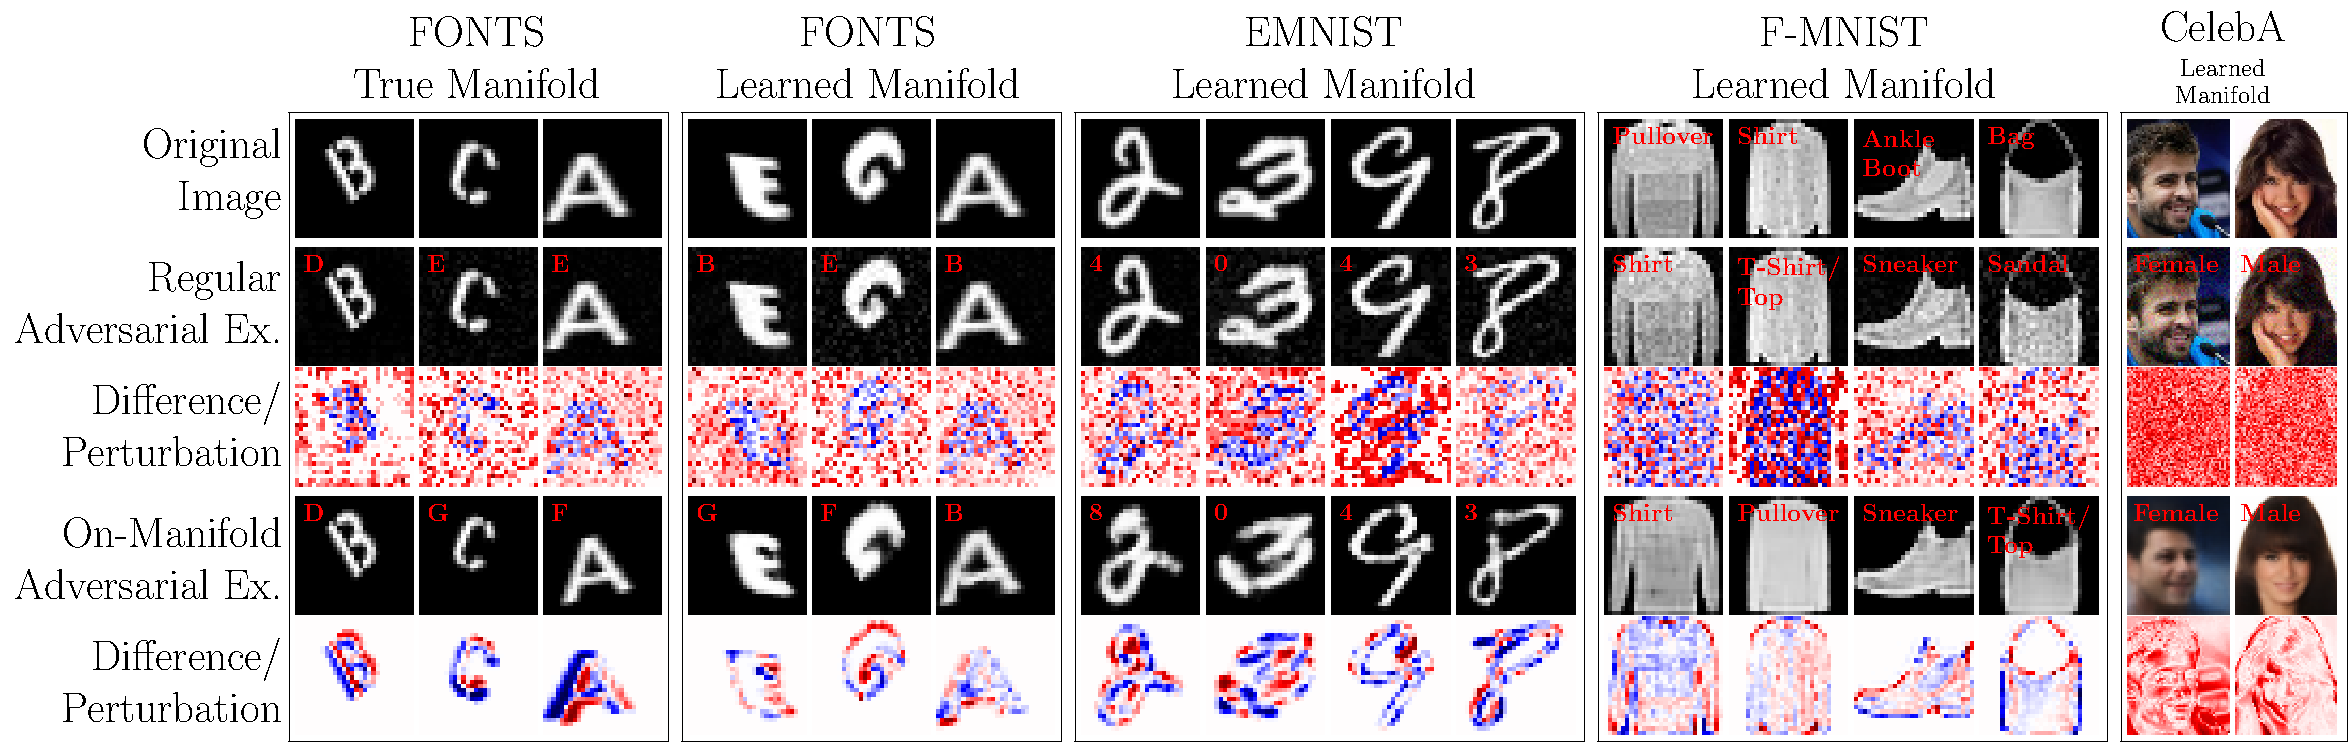
\includegraphics[width=1\textwidth]{main_examples.pdf}
    \vskip -6px 
    \caption{Regular and on-manifold adversarial examples on our synthetic dataset, \Fonts, consisting of randomly transformed characters ``A'' to ``J'', \MNIST \cite{CohenARXIV2017}, \Fashion \cite{XiaoARXIV2017} and \Celeb \cite{LiuICCV2015}. On \Fonts, the manifold is known by construction; in the other cases, the class manifolds have been approximated using \VAEGANs \cite{LarsenICML2016,RoscaARXIV2017}. The difference (normalized; or their magnitude on \Celeb) to the original test image reveals the (seemingly) random noise patterns of regular adversarial examples in contrast to reasonable concept changes of on-manifold adversarial examples.}
    \label{fig:main-examples}
\end{figure*}

\myparagraph{Attacks:} Adversarial examples for deep networks were first reported in \cite{SzegedyARXIV2013}; the problem of adversarial machine learning, however, has already been studied earlier~\cite{BiggioPR2018}. Adversarial attacks on deep networks range from white-box attacks \cite{SzegedyARXIV2013,GoodfellowARXIV2014,KurakinARXIV2016b,PapernotSP2016b,MoosaviCVPR2016,MadryICLR2018,CarliniSP2017,RoszaBMVC2017,DongCVPR2018,LuoAAAI2018}, with full access to the model (weights, gradients \etc), to black-box attacks \cite{ChenAISEC2017,BrendelARXIV2017a,SuARXV2017,IlyasARXIV2018,SarkarARXIV2017,NarodytskaCVPRWORK2017}, with limited access to model queries. White-box attacks based on first-order optimization, \eg, \cite{MadryICLR2018,CarliniSP2017}, are considered state-of-the-art. Due to their transferability \cite{LiuICLR2017,XieARXIV2018,PapernotASIACCS2017}, these attacks can also be used in a black-box setting (\eg using model stealing \cite{ShokriSP2017,PapernotASIACCS2017,TramerUSENIX2016,WangSP2018,OhICLR2018,JuutiARXIV2018}) and have, thus, become standard for evaluation. Recently, generative models have also been utilized to craft -- or learn -- more natural adversarial examples \cite{SongARXIV2018,BrownARXIV2018,ZhaoICLR2018,SchottARXIV2018}. Finally, adversarial examples have been applied to a wide variety of tasks, also beyond computer vision, \eg, \cite{FischerICLR2017,CisseNIPS2017,TabacofARXIV2016,KosSPWORK2018,HuangICLR2017,LinIJCAI2017,AlzantotEMNLP2018,CarliniWP2018}.

\myparagraph{Defenses:} Proposed defenses include detection and rejection methods \cite{GrosseARXIV2017,FeinmanARXIV2017,LiaoCVPR2018,MaARXIV2018,AmsalegWIFS2017,MetzenARXIV2017}, pre-processing, quantization and dimensionality reduction methods \cite{BuckmanICLR2018,PrakashDCC2018,BhagojiARXIV2017}, manifold-projection methods \cite{IlyasARXIV2017,SamangoueiICLR2018,SchottARXIV2018,ShenARXIV2017}, methods based on stochasticity/regularization or adapted architectures \cite{ZantedschiAISEC2017,BhagojiARXIV2017,NayebiARXIV2017,SimonGabrielARXIV2018,HeinNIPS2017,JakubovitzARXIV2018,RossAAAI2018,KannanARXIV2018,LambARXIV2018,XieICLR2018}, ensemble methods \cite{LiuARXIV2017,StraussARXIV2017,HeUSENIXWORK2017,TramerICLR2018}, as well as adversarial training \cite{ZantedschiAISEC2017,MiyatoICLR2016,HuangARXIV2015,ShahamNEUROCOMPUTING2018,SinhaICLR2018,LeeARXIV2017b,MadryICLR2018}; \red{however, many defenses have been broken, often by considering ``specialized'' or novel attacks \cite{CarliniAISec2017,CarliniARXIV2016,AthalyeARXIV2018b,AthalyeARXIV2018}}. In \cite{AthalyeARXIV2018}, only adversarial training, \eg, the work by Madry \etal \cite{MadryICLR2018}, has been shown to be effective -- although many recent defenses have not been studied extensively. Manifold-based methods, in particular, have received some attention lately: in \cite{IlyasARXIV2017,SamangoueiICLR2018}, generative adversarial networks \cite{GoodfellowNIPS2014} are used to project an adversarial example back to the learned manifold. Similarly, in \cite{SchottARXIV2018}, variational auto-encoders \cite{KingmaICLR2014} are used to perform robust classification.

\myparagraph{Generalization:} Research also includes independent benchmarks of attacks and defenses \cite{CarliniAISec2017,CarliniARXIV2016,AthalyeARXIV2018b,AthalyeARXIV2018,SharmaARXIV2017}, their properties \cite{LiuICLR2017,SharifARXIV2018}, as well as theoretical questions \cite{HeinNIPS2017,JakubovitzARXIV2018,FawziICMLWORK2015,TanayARXIV2016,GilmerICLRWORK2018,SimonGabrielARXIV2018,TsiprasARXIV2018,WangICML2018}. Among others, the existence of adversarial examples \cite{SzegedyARXIV2013,GoodfellowARXIV2014,TanayARXIV2016} raises many questions. While Szegedy \etal \cite{SzegedyARXIV2013} originally thought of adversarial examples as ``extremely'' rare negatives and Goodfellow \etal \cite{GoodfellowARXIV2014} attributed adversarial examples to the linearity in deep networks, others argued against these assumptions \cite{GilmerICLRWORK2018,TanayARXIV2016}. Instead, a widely accepted theory is the manifold assumption; adversarial examples are assumed to leave the data manifold \cite{GilmerICLRWORK2018,TanayARXIV2016,IlyasARXIV2017,SamangoueiICLR2018,SchottARXIV2018}.

This paper is particularly related to work on the connection of adversarial examples to generalization \cite{TsiprasARXIV2018,SuARXV2018,GilmerICLRWORK2018,RozsaICMLA2016}. Tsipras \etal \cite{TsiprasARXIV2018} and Su \etal \cite{SuARXV2018} argue that there exists an inherent trade-off between robustness and generalization. However, the theoretical argument in \cite{TsiprasARXIV2018} is questionable as adversarial examples are allowed to change their actual, true label \wrt the data distribution, as illustrated \figref{fig:introduction} (c). The experimental results obtained in \cite{SuARXV2018,RozsaICMLA2016} stem from comparing different architectures and training strategies; in contrast, we consider robustness and generalization for any arbitrary but fixed model. On a \red{simple} synthetic toy dataset, Gilmer \etal \cite{GilmerICLRWORK2018} show that on-manifold adversarial examples exist. We further show that on-manifold adversarial examples also exist on real datasets with unknown manifold, similar to \cite{ZhaoICLR2018}. \red{In contrast to \cite{GilmerICLRWORK2018,ZhaoICLR2018}, we utilize a gradient-based attack on the manifold, not in image space.} Our work is also related to \cite{FawziICIP2016} and \cite{MiyatoICLR2016,MiyatoPAMI2018} where variants of adversarial training are used to boost (semi-)supervised learning. While, \eg, Fawzi \etal \cite{FawziICIP2016}, apply adversarial training to image transformations, we further perform adversarial training on adversarial examples constrained to the true, or approximated, manifold. \red{This is also different from adversarial data augmentation schemes driven by GANs, \eg, \cite{RatnerNIPS2017,SixtFRAI2018,AntoniouICANN2018,CubukARXIV2018}, where training examples are generated, but without the goal to be mis-classified.} \red{Finally, \cite{SongICLR2018} provide experimental evidence that adversarial examples have low probability under the data distribution; we show that adversarial examples have, in fact, zero probability.}